\documentclass{article}
\usepackage{graphicx} % Required for inserting images
\usepackage{float}
\usepackage{biblatex}
\usepackage{hyperref}
\usepackage{letterspace}
\usepackage{setspace}
\setlength{\parskip}{4pt}
% \setstretch{1.5}
\graphicspath{{images/}}
\usepackage{listings}
\lstset{language=Java, basicstyle=\scriptsize}
\addbibresource{references.bib}
\title{COMP3100 \\ Client-Side Simulator \\ Stage 1  }
\author{Hasham Masood \\ 46463100}
\date{March 2023}

\begin{document}

\maketitle
\tableofcontents
\section{Introduction }
This report is concerned with providing a comprehensive overview of the development of this client-side simulator (ds-client) project. My client application was designed to run in conjunction with \textbf{\textls{ds-server}} which may be viewed at \href{https://github.com/distsys-MQ/ds-sim}{\emph{ds-sim repository.}} The \textbf{\textls{ds-server}} provides information pertaining to the servers whilst the client is responsible for job scheduling in any fashion it desires. In line with our specifications, we will be implementing \textit{Largest-Round-Robin} (LRR) algorithm. This algorithm will allow us to distribute jobs equally in a round-robin manner between the largest servers. In essence, our client should be able to perform a successful handshake, retrieve the server list, identify the largest server, and then schedule the jobs using \textit{LRR}. Throughout this paper, we will outline the system overview providing a high-level description of the system. We may also consider the design philosophies that were undertaken. Lastly, we will analyse the code and explain its implementation.

\section{System Overview}
As alluded to previously the \textbf{\textls{ds-server}} and \textbf{\textls{myClient}} are designed to complement one another. The client establishes a connection to the server where it initiates a handshake. It exchanges relevant information and then receives the list of servers. The client then identifies the largest server type based on the number of CPU cores it has. The indices of these servers are then stored within an \emph{ArrayList}. Upon retrieval of job information from the server, the client schedules them using \emph{Largest-Round-Robin}. Once the client receives acknowledgment of job completion it closes the connection.

\subsection*{Diagram Model}
The following diagram provides a basic overview of how the client and server communicate. It also serves to provide an example as to how jobs are scheduled using \emph{LRR}.

\begin{figure}[htbp]
  \begin{minipage}{1\textwidth}
    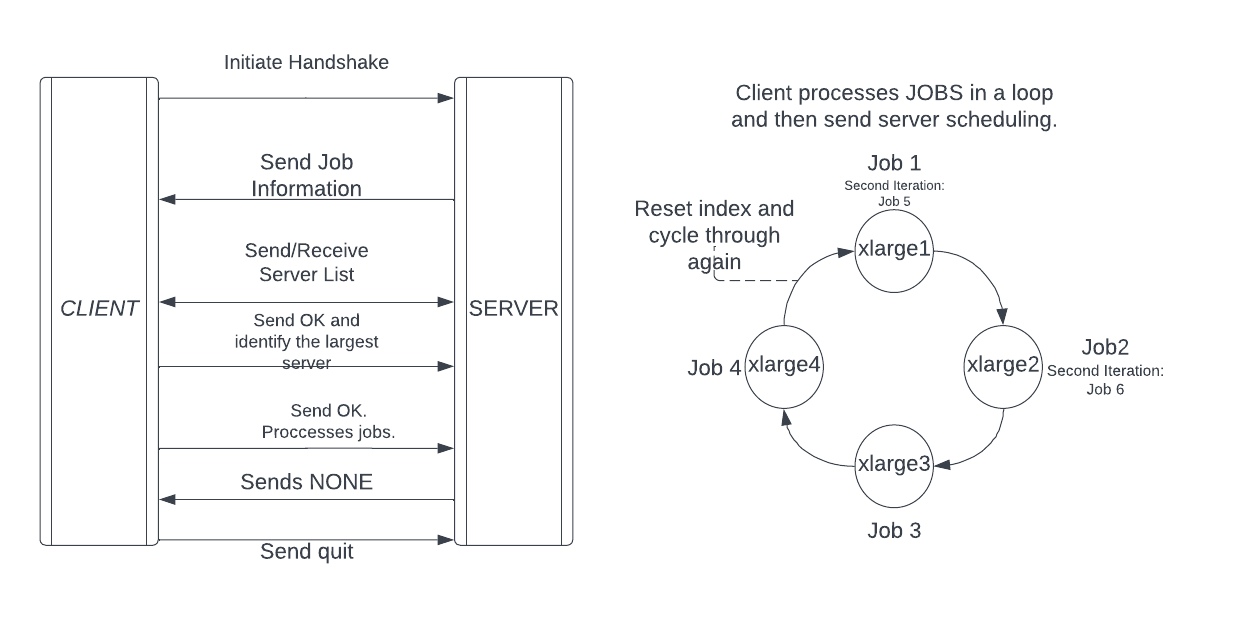
\includegraphics[width=\textwidth]{images/short3.png}
  \end{minipage}
  \hfill
  \begin{minipage}{1\textwidth}\raggedright
    \caption{Overview of \textbf{\textls{ds-server}} and \textbf{\textls{ds-client}} communication and LRR}
    \label{fig:image_label}
  \end{minipage}
\end{figure}

\section{Design }
Design philosophies are central to the development of any application. In the case of \textbf{\textls{myClient}} it was essential to first prioritise its successful operation. This resulted in no evidence of functional programming. This approach is quintessential in code maintenance as it allows code to be comprehensible and easier to edit in the future. This stands to be apparent in \emph{clientSend()} and \emph{ClientReceive()}. The former function is concerned with sending strings to the server using \textbf{DataOutputStream}. The latter is able to read the server's response from the \textbf{BufferedReader}. This is important in making the Handshake process read significantly clearer within the \emph{main()} function and removing a plethora of redundant code. This will likely remain an obstacle to continue traversing throughout stage one and subsequently, stage two.

Furthermore, when approaching the design for the method that would allow for the identification of the largest server it was apparent there were likely \emph{two} solutions. One might have invoked the use of an XML Parser as opposed to directly reading the server's output. I decided against using an XML Parser as a personal choice. However, its application may have seen some advantages by limiting server requests, and pre-processing might have made the process marginally faster. My experience with Java and object-orientated programming has made me familiar with \emph{ArrayLists} as opposed to XML parsing. Reading the \textbf{BufferedReader} and storing the sorted output within an ArrayList seemed the most sensible decision. This is because of their dynamic use-case, different configuration files present us with \emph{n} amount of servers and these \emph{ArrayLists} are re-sizable.

 In an experimental build, I designed a while loop that would send Gets All on every iteration. This effectively, made the client request the server information on every iteration. Which significantly strained the network overhead. By relocating \emph{GetsAll} and the \emph{LRR} scheduling outside the while loop the program became vastly more efficient. There was also another design constraint not accounted for on initial completion. There was no condition to check whether multiple largest server types with an identical number of cores existed. Its implementation vastly improves the accuracy of this program. The now non-existent constraints of experimental builds now allowed the while loop to consist exclusively of the components required for job scheduling. The \emph{LRR} scheduling works by scheduling a job to each server of the largest type and resetting its index each time all servers in the round-robin have received one job. This allows for a balancing workload between servers of this type.
  
\section{Implementation }
Let us now observe the implementation of all processes involved with the development of this client-side simulator. To begin, we may briefly note that imported libraries \emph{java.io}, \emph{java.net}, and \emph{java.ArrayLists}. The former two libraries are concerned with input/output and the latter is for \emph{ArrayLists} which we will be using to store our largest server indices. We then have class instances \textbf{Socket}, \textbf{DataOutputStream}, and \textbf{BufferedReader}. The almalgmation of these classes allow us to establish a connection to the server and both receive and send data across to and from it. This may be observed in the functions seen below:
\begin{lstlisting}
static void clientSend(String message) throws IOException {
    dout.write((message + "\n").getBytes());
    dout.flush();
      }
    
static String clientRead() throws IOException {
    String message = (String) dis.readLine();
    return message;
      }
\end{lstlisting}
As we progress to the \emph{Main()} method we may now observe the implementation of the \emph{handshake} which we have referenced prior in this paper. This consists of a series of messages sent to and from the server. We may observe how this process functions. The client initiates the exchange with "HELO", to which the server replies "OK". The client then sends "AUTH user.name", and the server responds with a welcome. The client then sends "REDY" and is then given a JOB i.e., JOBN 37 0 1135 2 500 2500. Client send GETS All and receive i.e., DATA 48 124. The first number proceeding DATA tells us the number of records. The client then sends "OK" to see the entire list of servers which will later be sorted.\newline

Let us now observe the string method \emph{split()} which we use extensively throughout this application. This method allows us to convert a string into an array and then retrieve a value at any given index. We may then employ the method \emph{parseInt()} which allows us to return an integer from the string array. This is seen below:

\begin{lstlisting}
      // Server sends: DATA 7 124 (number of records)
      String[] serverData = getsResponse.split(" ");
      int nRecs = Integer.parseInt(serverData[1]);
\end{lstlisting}

Succeeding this we use \emph{nRecs} within a for loop to iterate through our array and find the largest server type. The criteria for identifying this is on the basis of the number of CPU cores. Once we have split each server record into an array - we may parse the CPU value in Index 4. It then updates the \emph{LargestServerType} and \emph{LargestCPU}. The ArrayList stores the values and clears them when it finds a greater server type storing only the indices belonging to them. After running the shell-script from Week 6 workshop, I discovered that two servers may be of the largest type and hence, why the else conditional selects the first of the two types. This may be viewed below:

\begin{lstlisting}
for (int i = 0; i < nRecs; i++) {
    String serverInfo = (String) dis.readLine();
    String[] serverSplit = serverInfo.split(" ");
    int serverCPU = Integer.parseInt(serverSplit[4]);
    
    if (serverCPU > largestCPU) {
        largestServerType = serverSplit[0];
        largestCPU = serverCPU;
        largestServerList.clear();
        largestServerList.add(serverSplit[1]);
        } else if (serverCPU == largestCPU && serverSplit[0].equals(largestServerType)) {
        largestServerList.add(serverSplit[1]);
        }
    }
\end{lstlisting}

We then proceed to send OK to the Server and initiate our while loop that allows us to schedule the jobs using the LRR algorithm. If the server sends JOBN we schedule the job and send the schd command to the server. Once the currentIndex reaches the amount of servers denoted by the size of the ArrayList we use modulo to reset the counter to 0 and begin again. Thus achieveing our LRR quota, which may be observed in the previous figure.
\begin{lstlisting}
int currentIndex = 0;

while (true) {
    String[] jobReqSplit = jobRequest.split(" ");
    
    if (jobReqSplit[0].equals("JOBN") ) {
        int jobId = Integer.parseInt(jobReqSplit[2]);
        String serverInfo = largestServerList.get(currentIndex);
        String schdCommand = "SCHD " + jobId + " " + largestServerType + " " + serverInfo;
    
        dout.write((schdCommand + "\n").getBytes());
        dout.flush();
        currentIndex = (currentIndex + 1) % largestServerList.size();
        } else if (jobReqSplit[0].equals("NONE")) {
            break;
        }
\end{lstlisting}
Upon completion, the Server sends "NONE" signifying the completion of all jobs. This is the break condition for our while loop and thus, the last message the Client sends to the server is QUIT. This concludes the operation of my application and the end of this paper. 

\section{References }
[1]Hasham Masood, “Hashy01/COMP3100Project,” GitHub, Apr. 02, 2023. https://github.com/Hashy01/COMP3100Project 

[2]Y. Lee, “distsys-MQ/ds-sim,” GitHub, Feb. 28, 2023. https://github.com/distsys-MQ/ds-sim
\end{document}
